\documentclass[conference]{IEEEtran}

\usepackage{cite}
\usepackage{amsmath}
\usepackage{caption}
\usepackage{subcaption}
\usepackage{subcaption}
\usepackage[linesnumbered,ruled,vlined]{algorithm2e}
% Note that the amsmath package sets \interdisplaylinepenalty to 10000
% thus preventing page breaks from occurring within multiline equations. Use:
%\interdisplaylinepenalty=2500
% after loading amsmath to restore such page breaks as IEEEtran.cls normally
\usepackage{url}
\usepackage{hyperref}
\usepackage{verbatim}
\usepackage{siunitx}
\usepackage{listings}
\usepackage{mathtools}
\usepackage{float}

\lstdefinelanguage{Julia}{
  basicstyle=\small\ttfamily,
  showspaces=false,
  showstringspaces=false,
  keywordstyle={\textbf},
  morekeywords={if,else,elseif,while,for,begin,end,quote,try,catch,return,local,abstract,function,stagedfunction,macro,ccall,finally,typealias,break,continue,type,global,module,using,import,export,const,let,bitstype,do,in,baremodule,importall,immutable},
  escapeinside={~}{~},
  morecomment=[l]{\#},
%  commentstyle=\textsf,
  commentstyle={},
  morestring=[b]",
}

\lstset{language=Julia,basicstyle=\footnotesize\ttfamily,breaklines=true}

\DeclarePairedDelimiter\ceil{\lceil}{\rceil}
\DeclarePairedDelimiter\floor{\lfloor}{\rfloor}

% correct bad hyphenation here
\hyphenation{}


\begin{document}

\title{Automated benchmarking in noisy environments}

% author names and affiliations
% use a multiple column layout for up to three different
% affiliations
\author{\IEEEauthorblockN{Jiahao Chen and Jarrett Revels}
\IEEEauthorblockA{Computer Science and Artificial Intelligence Laboratory\\
Massachusetts Institute of Technology\\
Cambridge, Massachusetts 02139--4307\\
Email: \{jiahao,jrevels\}@csail.mit.edu}
}

% make the title area
\maketitle

%%%%%%%%%%%%%%%%%%%%%%%%%%%%%%%%%%%%%%%%%%%%%%%%%%%%%%%%%%%%%%%%%%%%%%%%%%%%%%%%%%%%%%%%%%%%
\begin{abstract}
We propose a benchmarking strategy that is robust in the presence of timer
error, OS jitter and other environmental fluctuations, and is insensitive to
the highly nonideal statistics produced by timing measurements.
We construct a model that explains how these strongly nonideal statistics can
arise from environmental fluctuations, and also justifies our proposed
strategy. We implement this strategy in the BenchmarkTools Julia package, where
it is used in production continuous integration (CI) pipelines for developing
the Julia language and its ecosystem.
\end{abstract}

\IEEEpeerreviewmaketitle

%%%%%%%%%%%%%%%%%%%%%%%%%%%%%%%%%%%%%%%%%%%%%%%%%%%%%%%%%%%%%%%%%%%%%%%%%%%%%%%%%%%%%%%%%%%%
\section{Introduction}
\label{sec:intro}

Authors of high performance applications rely on benchmark suites to detect and avoid
program regressions. However, many developers often run benchmarks and interpret their
results in an ad hoc manner with little statistical rigor. This ad hoc interpretation wastes
development time and can lead to misguided decisions that worsen performance.

In this paper, we consider the problem of designing a language- and
platform-agnostic benchmarking methodology that is suitable for continuous
integration (CI) pipelines and manual user workflows. Our methodology
especially focuses on the accommodation of benchmarks whose expected executions
times are short enough that timing measurements are vulnerable to error due to
insufficient system timer accuracy (generally on the order of microseconds or
shorter).

\subsection{Accounting for performance variations}
\label{sec:variations}

Modern hardware and operating systems introduce many confounding factors that complicate a
developer's ability to reason about variations in user space application
performance~\cite{HP5e}.\footnote{A summary of these factors can be found in the
\href{https://github.com/JuliaCI/BenchmarkTools.jl}{\lstinline|BenchmarkTools|}
documentation in the
\href{https://github.com/JuliaCI/BenchmarkTools.jl/blob/4db27210d43abf2c55226366f3a749afe1d64951/doc/linuxtips.md}{docs/linuxtips.md}
file.} Timing measurements can exhibit correlation structures that depend on a myriad of
factors such as environment temperature, workload, power availability, and network traffic,
and operating system (OS) configuration. These factors are the subject of much existing
research on system quiescence, where the aim is to identify and control for sources of
variation in program runtime measurements.

A large number of these sources stem from OS behavior, including CPU frequency scaling
\cite{RHEL6}, address space layout randomization (ASLR)~\cite{Shacham2004}, virtual memory
management~\cite{Oyama2014,Oyama2016}, differences between CPU privilege
levels~\cite{Zaparanuks2009}, context switches due to interrupt handling~\cite{Tsafrir2007},
activity from system daemons and cluster managers~\cite{Petrini2003}, and suboptimal
process- and thread-level scheduling~\cite{Lozi2016}. Even seemingly irrelevant
configuration parameters like the size of the OS environment can confound experimental
reproducibility by altering the alignment of data in memory~\cite{Mytkowicz2009}. Other
sources of variation come from specific language features or implementation details. For
example, linkers for many languages are free to choose the binary layout of the library or
executable arbitrarily, resulting in non-deterministic memory layouts~\cite{Georges2008}.
This problem is exacerbated in languages like C++, whose compilers introduce arbitrary name
mangling of symbols~\cite{Kalibera2005}. Overzealous compiler optimizations can also
adversely affect the accuracy of hardware counters~\cite{Zaparanuks2009}, or in extreme
cases eliminate key parts of the benchmark as dead code. Yet another example is garbage
collector performance, which is influenced from system parameters such as heap
size~\cite{Blackburn2004}.

\subsection{Statistics of timing measurements are not i.i.d.}
\label{sec:toughstats}

\begin{figure}
\centering
\begin{subfigure}{0.22\textwidth}
    \centering
    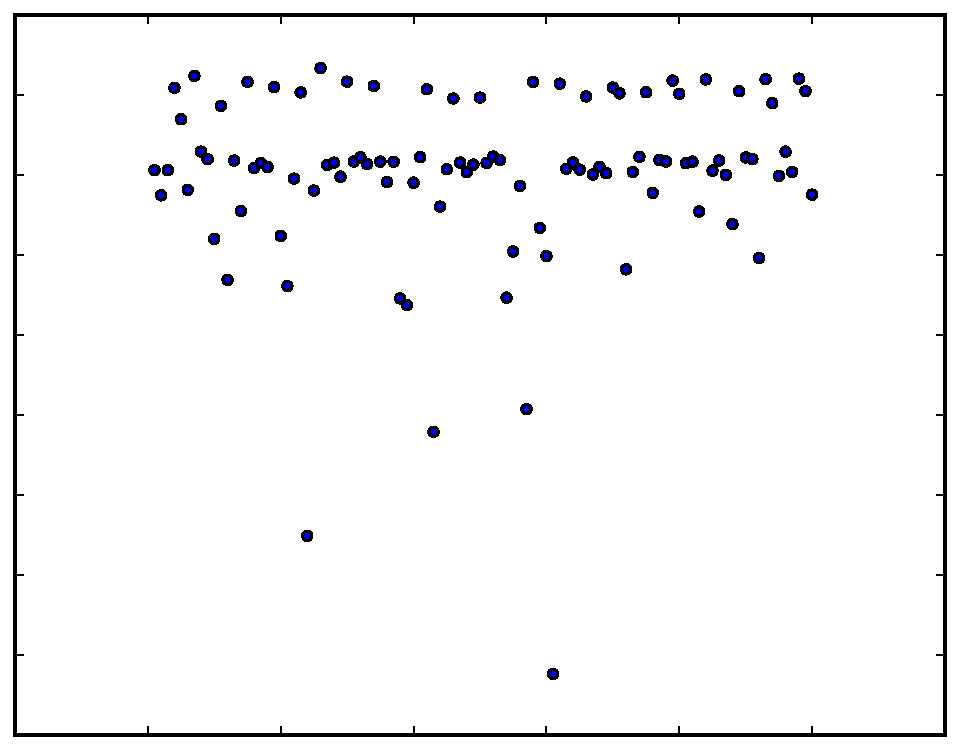
\includegraphics[width=\textwidth]{figures/fig1/simple_branchsum_fast}
    \caption{Benchmark 1: Unimodal with skew and large outliers}
\end{subfigure}%
~
\begin{subfigure}{0.22\textwidth}
    \centering
    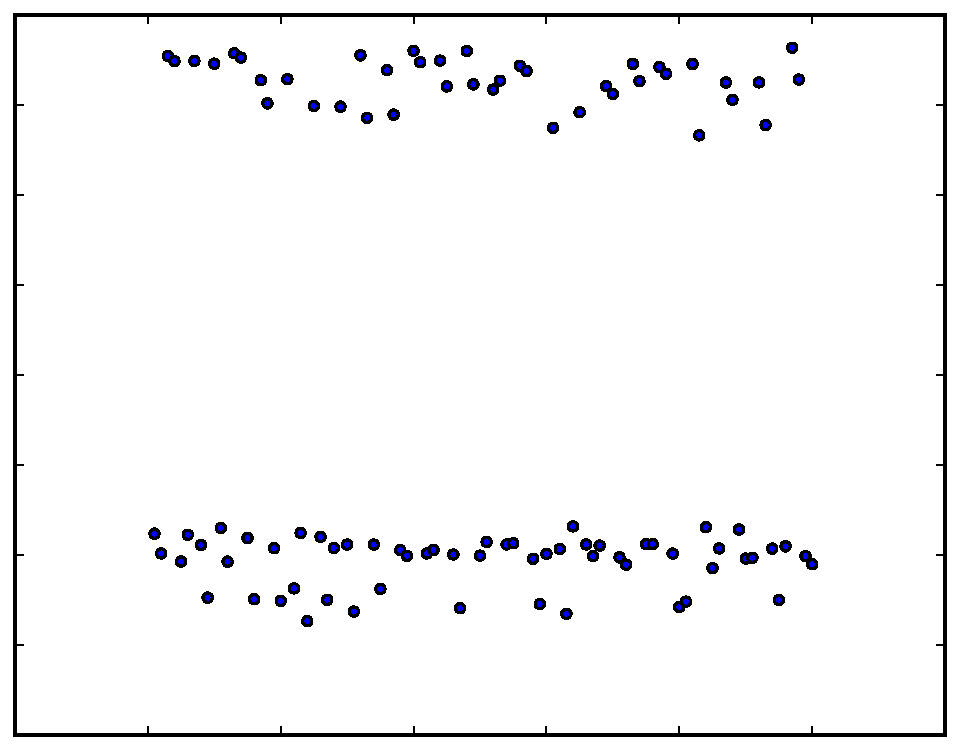
\includegraphics[width=\textwidth]{figures/fig1/bimodal_branchsum}
    \caption{Benchmark 2: Bimodal}
\end{subfigure}
\begin{subfigure}{0.22\textwidth}
    \centering
    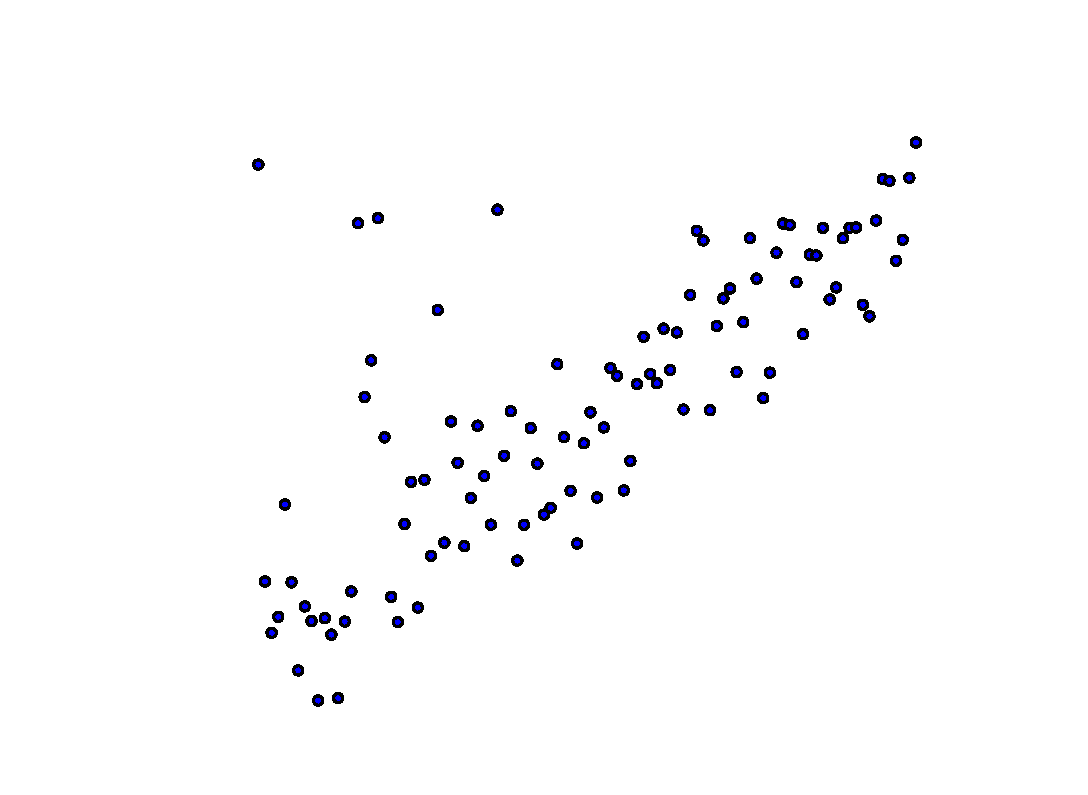
\includegraphics[width=\textwidth]{figures/fig1/drift_manyallocs_slow}
    \caption{Benchmark 3: Drift}
\end{subfigure}
~
\begin{subfigure}{0.22\textwidth}
    \centering
    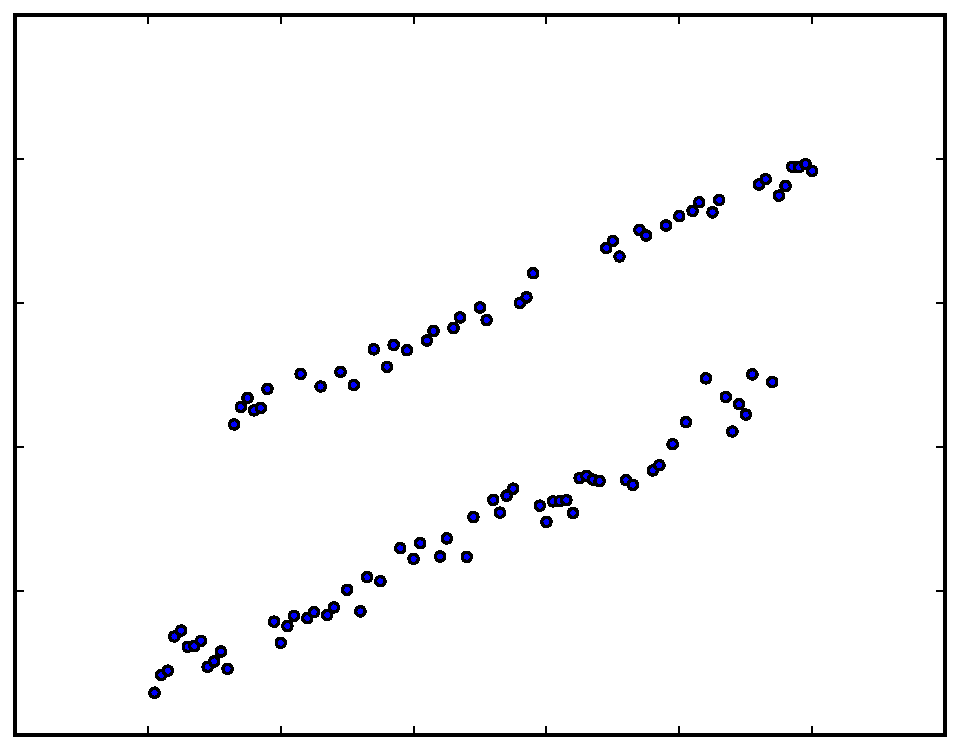
\includegraphics[width=\textwidth]{figures/fig1/bimodal_drift_sumindex}
    \caption{Benchmark 4: Bimodal with drift}
\end{subfigure}
\caption{Variability in the mean benchmark time across multiple trials, showing
that the mean has non-i.i.d., non-normal behavior in four different benchmarks.
Each point represents a mean time computed from trial of 10,000 measurements.
The horizontal axis is the index of the trial, while the vertical axis is time.}
\label{fig:meandistributions}
\vspace{-0.45cm} % hack to get rid of weirdly large line gap below this figure
\end{figure}

The myriad sources of performance variation result in timing measurements that are not
always independent and identically distributed (i.i.d). Many textbook statistical approaches
fail in this case due to a reliance on the central limit theorem, which does not generally
hold in the non-i.i.d. regime. Empirical program timing distributions are also often
heavy-tailed, and hence contain many outliers.

The violation of the central limit theorem can be seen empirically in many Julia benchmarks.
For example, Figure~\ref{fig:meandistributions} shows that none of the four illustrative
benchmarks considered in this paper exhibit normality in the sample mean. Instead, we see
that the mean demonstrates skewed density and outliers in the first benchmark, bimodality in
the second and fourth benchmarks, and upward drift in the third and fourth benchmarks.

Many other authors have also noted the lack of textbook statistical behavior in timing
measurements~\cite{Gil2011,Chen2015,Rehn2015,Barrett2016}. Authors have also noted the poor
stastistical power of standard techniques such as $F$-tests or Student t-tests for benchmark
timings~\cite{Lilja2000,Mytkowicz2009,Kalibera2013,Chen2015,Barrett2016}. Parametric outlier
detection techniques, such as the 3-sigma rule used in benchmarking software like
\lstinline|AndroBench|\cite{Kim2012}, can also fail when applied to non-i.i.d. timing measurements.

There is a lack of consensus over how non-ideal timing measurements should be treated. Some
authors propose automated outlier removal and analyzing the remaining bulk
distribution~\cite{Kim2012}; however, these methods run the risk of fundamentally distorting
the true empirical distribution for the sake of normal analysis. Other authors have proposed
purposely introducing randomness in the form of custom OS kernels
\cite{Tessellation,Akkan2012}, custom compilers providing reproducible~\cite{Georges2008} or
consistently randomized~\cite{Curtsinger2013} binary layouts, or low-variability garbage
collectors~\cite{Huang2004}. Unfortunately, these methods are specific to a single
programming language, implementation, and/or platform. Furthermore, these methods often
require administrative privileges and drastic modifications to the benchmarking environment,
which are impractical demands for automated benchmarking software to make of the user.

\subsection{Existing benchmarking methodologies}
\label{sec:existingtools}

While it is impossible to eliminate performance variation
entirely~\cite{Alcocer2015,Barrett2016}, benchmarking methodologies that attempt to account
for both measurement error and external sources of variation do exist. For example, the
Haskell microbenchmarking package \lstinline|criterion|~\cite{criterion} attempts to thwart
error due to timer inaccuracy by growing the number of benchmark executions per timing
measurement as more timing measurements are obtained. After all measurements are taken, a
summary estimate of the benchmark runtime is obtained by examining the derivative of the
ordinary least squares regression line at the point of a single evaluation point. There are
three disadvantages to this approach. First, the least squares fit is sensitive to
outliers~\cite{Maronna2006} (though \lstinline|criterion| does warn the user if outliers are
detected) Second, measurements made earlier in this experiment are highly vulnerable to
timer error, since few benchmark repetitions are used. These early measurements can skew the
regression, and hence also skew the final runtime estimate. Third, measurements made later in
the experiment can repeat the benchmark more times than are necessary to overcome timer
error, constituting an inefficient use of experiment time.

Another approach focuses on figuring out how many benchmark executions are required before
timing measurements of the benchmark become i.i.d.~\cite{Kalibera2013}. Their approach is
largely platform-agnostic, recognizes the pitfalls of inter-measurement correlations, and
acknowledges that merely increasing the number of benchmark repetitions is not always a
sufficient strategy to yield i.i.d. samples. However, the methodology focuses on mean-based
estimators, which are sensitive to outliers. Furthermore, the authors do not report if their
statistical tools generate correct confidence intervals. The moment-corrected formulae
described are accurate only for near-normal distributions, which is unlikely to hold for the
kinds of distributions we observed in real world statistics. Additionally, the methodology
requires a manual calibration experiment to be run for each benchmark, compiler, and
platform combination. As a result, this method is is difficult to automate on the scale of
Julia's standard library benchmark suite, which contains over 1300 benchmarks, and is
frequently expanded to improve performance test coverage.

Below, we describe our methodology to benchmarking for detecting performance regressions,
and how it is justified from a microscopic model for variations in timing measurements. To
the best of our knowledge, our work is the first benchmarking methodology that can be fully
automated, is robust in its assumption of non-i.i.d. timing measurement statistics, and
makes efficient use of a limited time budget.

%%%%%%%%%%%%%%%%%%%%%%%%%%%%%%%%%%%%%%%%%%%%%%%%%%%%%%%%%%%%%%%%%%%%%%%%%%%%%%%%%%%%%%%%%%%%
\section{Terms and definitions}
\label{sec:notation}

\begin{itemize}
    \item
    $P_0$, $P$ and $Q$ denote \textbf{benchmarkable programs}, each defined by
    a tape (sequence) of instructions.

    \item
    $I^{[i]}_{P}$ is the $i^{\textrm{th}}$ \textbf{instruction} in the tape
    defining program $P$.
    Instructions are indexed in bracketed superscripts, $\cdot^{[i]}$.

    \item
    $D^{[i]}_{P}$ is the \textbf{delay instruction} associated with $I^{[i]}_{P}$.
    Delay instructions are defined in Sec.~\ref{sec:model}.

    \item
    $T_i$ is a \textbf{timing measurement}, namely the amount of time taken to
    perform $n_i$ \textbf{executions} of a benchmarkable program. This quantity
    is directly measurable in an experiment.

    \item
    $t$ is a \textbf{theoretical execution time}.
    $t_{P_0}$ is the minimum time required to perform a single execution of
    $P_0$ on a given computer.

    \item
    \textbf{Estimated quantities} are denoted with a hat, $\hat\cdot$.
    For example, $\hat{t}_{P_0}$ is an estimate of the theoretical execution
    time $t_{P_0}$.

    \item
    A benchmark \textbf{experiment} is a recipe for obtaining multiple timing
    measurements for a benchmarkable program. Experiments can be executed to
obtain \textbf{trials}. The
    $i^{\textrm{th}}$ trial of an experiment is a collection of timing measurements
    $T^{\{i\}}_1, \dots T^{\{i\}}_j, \dots T^{\{i\}}_k$. Trial indices are always
    written using embraced superscripts, $\cdot^{\{i\}}$.

    \item
    $\tau$ denotes time quantities that are external to the benchmarkable program:
    \begin{itemize}
        \item $\tau_{\textrm{budget}}$ is the \textbf{time budget} for an experiment.
        \item $\tau_{\textrm{acc}}$ is the \textbf{accuracy} of the system timer, i.e.\ an upper bound on the maximal error in using the system timer to time an experiment.
        \item $\tau_{\textrm{prec}}$ is the \textbf{precision} of the system timer, namely the smallest nonzero time interval measurable by the timer.
    \end{itemize}

    \item
    $x_P^{(i)[j]} \tau^{(i)}$ is the \textbf{time delay} due to the
    $i^{\textrm{th}}$ \textbf{delay factor} for delay instruction $D^{[j]}$.  Specifically,
    $\tau^{(i)}$ is the factor's \textbf{time scale} and $x_P^{(i)[j]}$ is the factor's
    \textbf{trigger coefficient}, as introduced Sec.~\ref{sec:model}. Delay factors are indexed with  parenthesized
    superscripts, $\cdot^{(i)}$.

    \item
    $\epsilon$ is the measurement error due to timer inaccuracy.

    \item
    $E_m = \frac{T_m}{n_m} - t_{P_0}$ is the total contribution of all delay
factors found in measurement $m$, plus the measurement error $\epsilon$.

    \item
    $X^{(i)}_P$ is the \textbf{total trigger count} of the $i^{\textrm{th}}$
    delay factor during the execution of program $P$.

    \item
    $\nu$ is an \textbf{oracle function} that, evaluated at an execution time
$t$, estimates an appropriate $n$ necessary to overcome measurement error due
to insufficient
    $\tau_{\textrm{acc}}$ and $\tau_{\textrm{prec}}$. The oracle is described in detail in Sec.~\ref{sec:oracle}.
\end{itemize}

%%%%%%%%%%%%%%%%%%%%%%%%%%%%%%%%%%%%%%%%%%%%%%%%%%%%%%%%%%%%%%%%%%%%%%%%%%%%%%%%%%%%%%%%%%%%
\section{A model for benchmark timing distributions}
\label{sec:model}

We now present a statistical description of benchmark behavior which avoids the problematic
assumption that timing measurments are i.i.d. We will use this model later to justify the
design of a new automated experimental procedure.

\subsection{User benchmarks run with uncontrollable delays}
\label{sec:programmodel}

Let $P_0$ be a deterministic benchmark program which consists of an instruction tape
consisting of $k$ instructions:
%
\begin{equation}
    P_0 = \left[I^{[1]}, I^{[2]}, \dots I^{[k]}\right]
\end{equation}
%
Let $\tau^{[i]}$ be the runtime of instruction $I^{[i]}$. Then, the total run
time of $P_0$ can be written $t_{P_0} = \sum_{i=1}^N \tau^{[i]}$.

While a computer may be directed to execute $P_0$, it may not necessarily run the program's
instructions as they are originally provided. Recall that the environment in which $P_0$
runs is vulnerable to the factors described earlier in Sec.~\ref{sec:variations}. Crucially,
these factors only \textit{delay} the completion of the original instructions, rather than
speed them up.\footnote{While there are a very few external factors which might speed up
program execution, such as frequency scaling~\cite{RHEL6}, they can be easily accounted for
by ensuring that power consumption profiles are always set for maximal performance. We
therefore assume that these factors have been accounted for.} Therefore, we refer to them as
\textit{delay factors}. We can incorporate these delay factors into our description by
modeling their effects as extra instructions which, when interleaved with the original
instructions, do not change the semantics of $P_0$, but still add to the program's total
runtime. Thus, we can define a new program $P$ which consists of $P_0$'s original
instructions interleaved with additional \textit{delay instructions} $D^{[i]}$:
%
\begin{equation}
    P = \left[I^{[1]}, D^{[1]}, I^{[2]}, D^{[2]}, \dots I^{[k]}, D^{[k]}\right]
\end{equation}
%
The runtime of $P$ can then be written
%
\begin{equation}
    t_P = t_{P_0} + \sum_{i} \tau^{[i]}_D
\end{equation}
%
where $\tau^{[i]}_D$ is the execution time of $D^{[i]}$. Since $\tau^{[i]}_D \ge 0$, it
follows that $t_P \ge t_{P_0}$.

Each $\tau^{[i]}_D$ can be further decomposed into the runtime contributions of
individual delay factors. Let us imagine that each delay factor $j$ can either
contribute or not contribute to $D^{[i]}$. Assuming that each delay factor
triggers inside $D^{[i]}$ with constant probability $p^{[i](j)}$ of taking a
fixed time $\tau^{(j)}$, we can then write:
%
\begin{equation}
    \tau^{[i]}_D = \sum_{i} x_P^{[i](j)} \tau^{(j)}
\end{equation}
%
where $x_P^{[i](j)}$ is a Bernoulli random variable with success probability $p^{[i](j)}$.
We denote the total number of times the $i^{\textrm{th}}$ delay factor was triggered during
the execution of $P$ as the \textit{trigger count} $X_P^{(i)} = \sum_{j} x_P^{[i](j)}$.
Since the trigger count is a sum of independent Bernoulli random variables with nonidentical
success probabilities, $X_P^{(j)}$ is itself a random variable that follows a Poisson
binomial distribution parameterized by the success probabilities $\left[p^{(1)[j]}, \dots
p^{(k)[j]}\right]$. Our final expression for $t_P$ in terms of these quantities is then:
%
\begin{align}
t_P &= t_{P_0} + \sum_{i=1}^{k} \tau^{[i]}_D \nonumber \\
    &= t_{P_0} + \sum_{i=1}^{k} \sum_{j} x_P^{[i](j)} \tau^{(j)} \nonumber \\
    &= t_{P_0} + \sum_{j} X_P^{(j)} \tau^{(j)}.
\end{align}
%
In summary, our model treats $t_P$ as a random variable whose distribution
depends on the trigger probabilities $p^{[i](j)}$, which are determined by the
combined behavior of the delay factors and the initial benchmark program $P_0$.

\subsection{Repeated benchmark execution is often necessary but not always sufficient}
\label{sec:measuremodel}

As mentioned in Sec.~\ref{sec:existingtools}, experiments which measure program
performance usually incorporate multiple benchmark executions to obtain more
accurate measurements. We now apply our model to show that multiple executions
are necessary to eliminate error due to timer inaccuracy, but are insufficient
to obviate the effects of delay factors.

Represent $n$ executions of the program $P_0$ comprised of $k$ instructions as
a single execution of a program $Q_0$, which is the result of concatenating $n$
copies of $P_0$:
%
\begin{align}
Q_0 &= \left[P_0, P_0, \dots P_0 \right] \nonumber \\
    &= \left[I_{P}^{[1]}, \dots I_{P}^{[k]}, I_{P}^{[1]}, \dots I_{P}^{[k]}, I_{P}^{[1]}, \dots I_{P}^{[k]} \right] \nonumber \\
    &= \left[I_{Q}^{[1]}, I_{Q}^{[2]}, \dots I_{Q}^{[nk]} \right],
\end{align}
%
with $I_{P}^{[i]} = I_{Q}^{[i + ck]}$ for $c \in \{0, \dots n - 1\}$.

Now interleave delay instructions as before to obtain the program $Q$ that is actually
executed. $Q$ is \textit{not} simply $n$ repetitions of $P$, since the delay instructions in
$Q$ are not simply copies of the delay instructions in $P$. An observed timing measurement
$T$ of a single execution of $Q$ can be decomposed as:
%
\begin{align}
    T &= t_{Q} + \epsilon \\ \nonumber
      &= t_{Q_0} + \sum_{j} X_Q^{(j)} \tau^{(j)} + \epsilon \\ \nonumber
      &= n \, t_{P_0} + \sum_{j} \sum_{i=1}^{nk} x_Q^{[i](j)} \tau^{(j)} + \epsilon
\end{align}
%
where $\epsilon$ is the error due to timer inaccuracy (whose magnitude must by definition be smaller than $\tau_\textrm{acc}$).

We may try to determine $t_{P_0}$ from the experimental time as $T/n$, which is
also the gradient of a linear model for $T$ against $n$ when the intercept is
zero. However, our model gives:
%
\vspace{-0.10cm}
\begin{equation}
    \frac{T}{n} = t_{P_0} + \frac{\sum_{j} \sum_{i=1}^{nk} x_Q^{[i](j)} \tau^{(j)} + \epsilon}{n}
\end{equation}
%
All the terms on the right hand side other than $t_{P_0}$ constitute the
error $E$ in our measurement. For large $n$, the term $\epsilon/n$ arising from
timer inaccuracy becomes negligible, but the behavior of the other term depends
on the specific structure of the delay factors. In the best case, each delay
factor triggers $o(n)$ times, so that $T/n\to t_{P_0}$ as desired. However, in
the worst case, where every factor triggers on every instruction, $x_Q^{[i](j)}
= 1$, and the large $n$ behavior of $T/n$ does not reduce to the true runtime
$t_{P_0}$, but instead:
%
\begin{equation}
\label{eq:11}
    \lim_{n\to\infty} \frac{T}{n} = t_{P_0} + k \sum_{j} \tau^{(j)}.
\end{equation}

\eqref{eq:11} is a key result of our model: One cannot reliably eliminate the
effects of external variations simply by executing the benchmark a large number
of times. Whether or not increasing $n$ can render the delay factor term
negligible depends entirely on the random variables $X_Q^{(j)}$, which,
recalling our discussion in Sec.~\ref{sec:variations}, are not easily
controlled in practice. Therefore, we can only expect that $T/n$ at large $n$
gives us at best an \textit{overestimate} of the true runtime $t_{P_0}$.

%%%%%%%%%%%%%%%%%%%%%%%%%%%%%%%%%%%%%%%%%%%%%%%%%%%%%%%%%%%%%%%%%%%%%%%%%%%%%%%%%%%%%%%%%%%%
\section{An automated procedure for configuring performance experiments}
\label{sec:confexperiment}

In this section, we present an experimental procedure for automatically selecting useful
values of $n$ for a given benchmark program. Our procedure estimates a value for $n$ which
primarily minimizes timer error and secondarily maximizes the number of measurements
obtainable within a given time budget.

\subsection{An algorithm for estimating the optimal $n$ value}

Given $P_0$ and a total time budget $\tau_{\textrm{budget}}$, we use the automatable
procedure in Alg.~\ref{alg:tuning} for guessing the minimum value of $n$ required to
overcome error due to timer inaccuracy. The algorithm makes use of an oracle function $\nu$,
which is discussed in greater detail below in Sec.~\ref{sec:oracle}.

\begin{algorithm}
    \caption{Estimating $n$, the optimal number of benchmark repetitions required to
    minimize timer error and maximize the number of data points obtainable within a
    time budget.}
    \label{alg:tuning}
    \KwIn{$P_0$, $\tau_{\textrm{acc}}$, $\tau_{\textrm{prec}}$, an oracle function $\nu : t \to n$}
    \KwOut{$n$}
    Let $j = \tau_{\textrm{acc}} / \tau_{\textrm{prec}}$.

    For $i \in \{1, \dots j\}$, measure the amount of time it takes to perform $i$
    executions of $P_0$, resulting in a collection of timing measurements $T_1, \dots T_j$.

    Estimate $t_{P_0}$ as $\hat{t}_{P_0} = \textrm{min}(\frac{T_1}{1}, \dots \frac{T_j}{j})$.

    Evaluate $\nu(\hat{t}_{P_0})$ to obtain $n$. Details of $\nu$ are given in Sec.~\ref{sec:oracle}
\end{algorithm}

The upper bound $j$ in Alg.~\ref{alg:tuning} is determined by the ratio of
timer accuracy to timer precision. If each timing measurement consists of more
than $j$ repetitions, then the contribution of timer inaccuracy to the total
error is less than $\tau_\textrm{acc} / j = \tau_\textrm{prec}$, and so is too
small to measure. Thus there is no reason to pick $n > j$. In practice,
$\tau_\textrm{acc}$ need only be an overestimate for the timer accuracy,
which would raise the $n$ determined, but is still an acceptable result.

Alg.~\ref{alg:tuning} need only be applied once per benchmark, since the
estimated $n$ can be cached for use in subsequent experiments on the same
machine. Thus, we consider this algorithm an automated preprocessing step that
does not count against our time budget $\tau_{\textrm{budget}}$. In this
regard, our approach differs significantly from other approaches like
\lstinline|criterion|, which
determines $n$ every time a benchmark is run.

\subsection{Justifying the minimum estimator}
\label{sec:minimum}

\begin{figure}
\centering
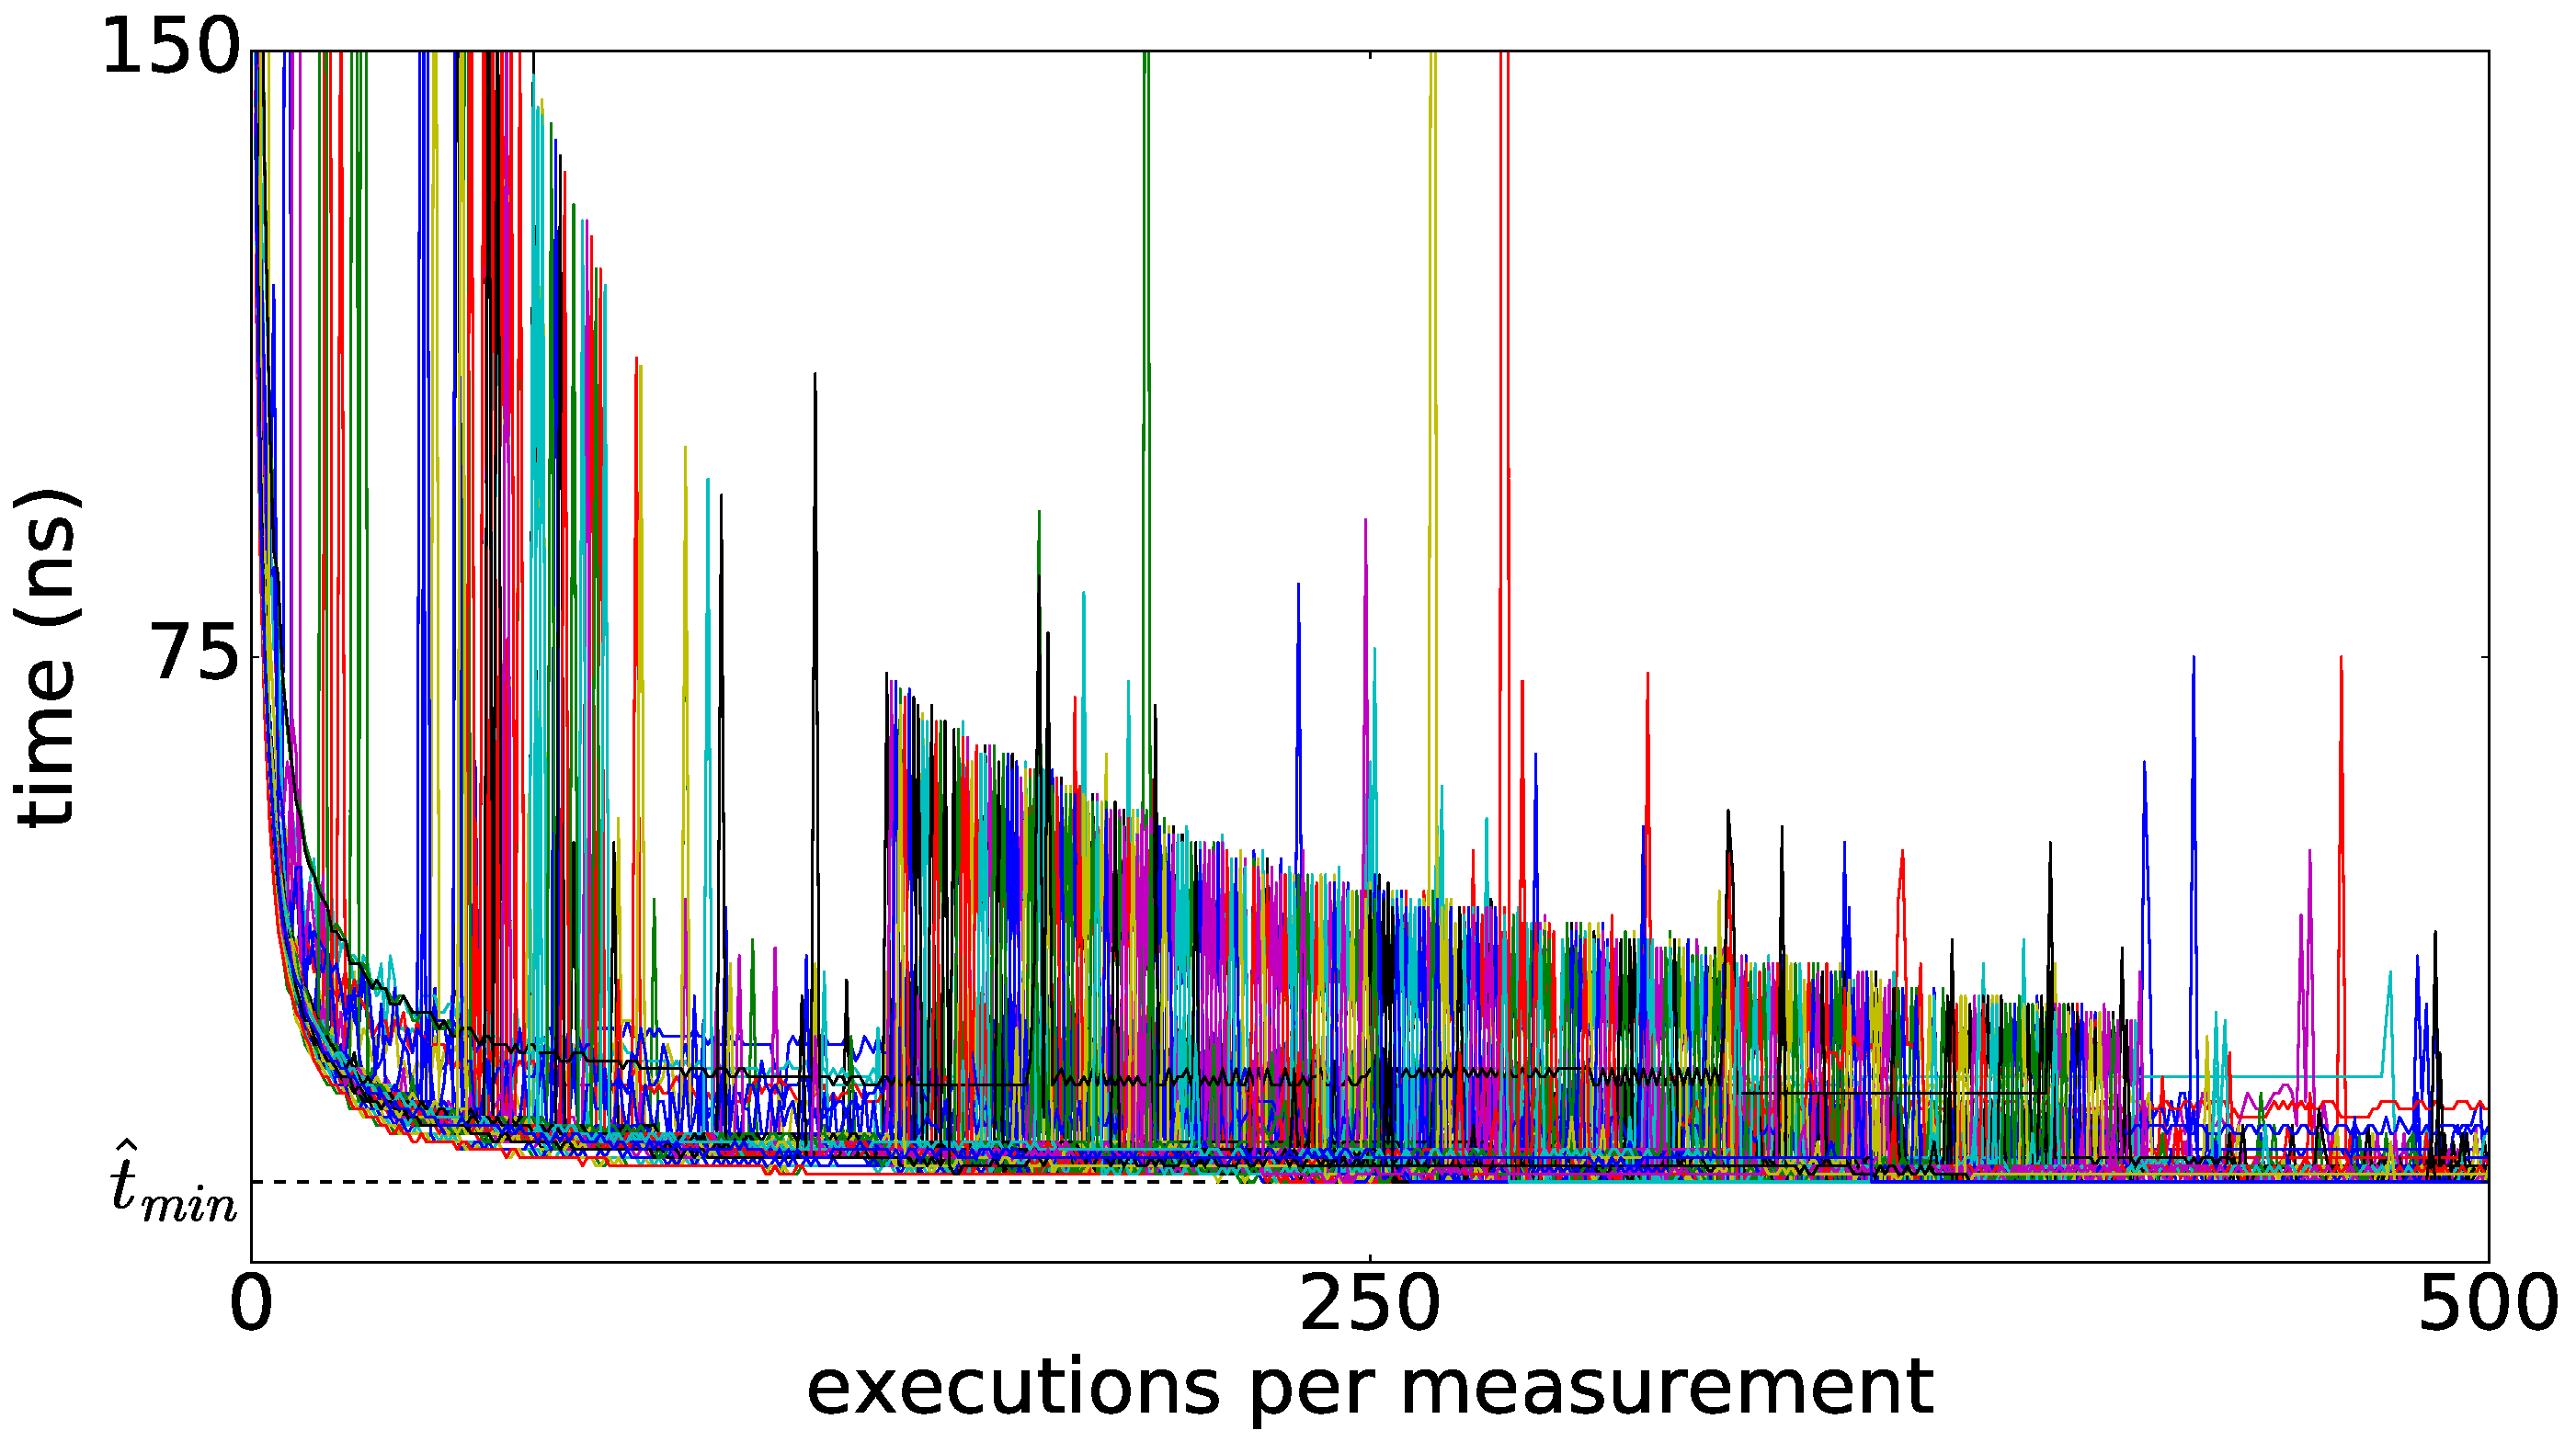
\includegraphics[width=\columnwidth]{figures/fig2/linear_scan_branchsum}
\caption{Plots of $T/n$ vs.\ $n$ produced by repeated experiments, each
consisting of running Alg.~\ref{alg:tuning} on the \lstinline|branchsum|
benchmark. While each experiment can produce wildly oscillatory curves, the
minimum across all the curves at each $n$ is much smoother and asymptotically
tends toward the same constant value.}
\label{fig:scaling}
\end{figure}

We will now justify Alg.~\ref{alg:tuning}'s use of the minimum to estimate $t_{P_0}$, as
opposed to the more common median or mean.

Consider the total error term for a given timing measurement $E_m = \frac{\left(\sum_{i}
X_Q^{(i)} \tau^{(i)} + \epsilon \right)_m}{n_m}$, such that $\frac{T_i}{n_i} = t_{P_0} +
E_i$. The minimum estimator applied to our timing measurements can then be written:

\begin{align}
    \hat{t}_{P_0} &= \textrm{min}(\frac{T_1}{1}, \dots \frac{T_j}{j}) \\ \nonumber
                  &= \textrm{min}(t_{P_0} + E_1, \dots t_{P_0} + E_j) \\ \nonumber
                  &= t_{P_0} + \textrm{min}(E_1, \dots E_j) \\ \nonumber
\end{align}

Thus, $\hat{t}_{P_0}$ is the estimate of $t_{P_0}$ which minimizes the error terms appearing
in our sample.

In the limit where the delay factor time scales are greater than $\tau_{\textrm{acc}}$, the
total error terms will always be positive, such that choosing the smallest timing
measurement will choose the sample with the smallest magnitude of error. If the delay factor
time scales are less than $\tau_{\textrm{acc}}$, choosing the smallest timing measurement
might choose a sample which underestimates $t_{P_0}$ due to negative timer error. In this
case, Alg.~\ref{alg:tuning} will simply pick a larger $n$ than is strictly necessary, which
is still acceptable.

\begin{figure}
\centering
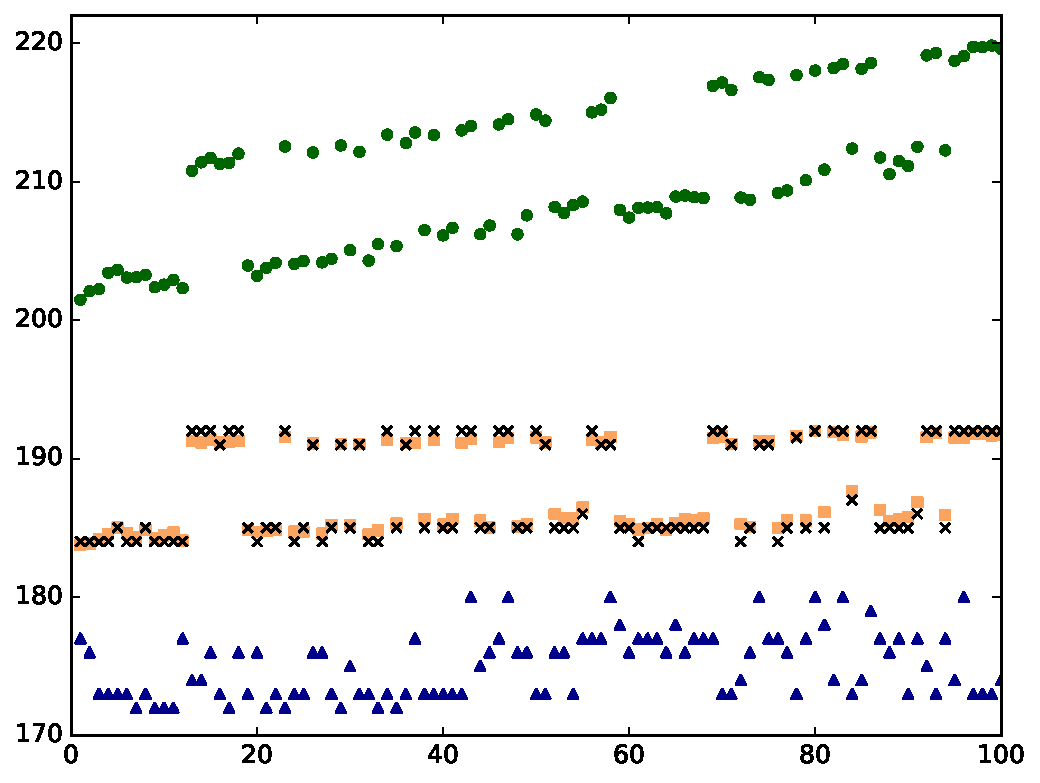
\includegraphics[width=\columnwidth]{figures/fig3/location_estimators_sumindex}
\caption{The behavior of different location parameters across multiple trials of
the \lstinline|sumindex| benchmark: mean (green filled circles), trimmed mean of
the 5th---95th percentiles (brown filled squares), median (black crosses), and
minimum (blue filled triangles).}
\label{fig:locationmeasures}
\end{figure}

Figs.~\ref{fig:locationmeasures} and \ref{fig:pdfsumindex} provide further
justification for the minimum over other common estimators like the median,
mean, or trimmed mean. Recall from Section~\ref{sec:model} that the $E_i$ terms
are sampled from a sum of scaled random variables following nonidentical
Poisson binomial distributions. As such, these terms often exhibit multimodal
behavior. While estimators like the median and trimmed mean are known to be
robust to outliers~\cite{Maronna2006}, Fig.~\ref{fig:locationmeasures}
demonstrates that they still capture bimodality of the distributions plotted in
Fig.~\ref{fig:pdfsumindex}. Thus, these estimators are undesirable because our
choice of $n$ could vary drastically between different executions of
Alg.~\ref{alg:tuning}, depending on which of the estimator's
modes was captured in the sample.  In contrast, the distribution of
the minimum across all experimental trials is always unimodal. Thus for our
purposes, the minimum is a unimodal, robust estimator for the location
parameter of a given benchmark's timing distribution.

\begin{figure}
\centering
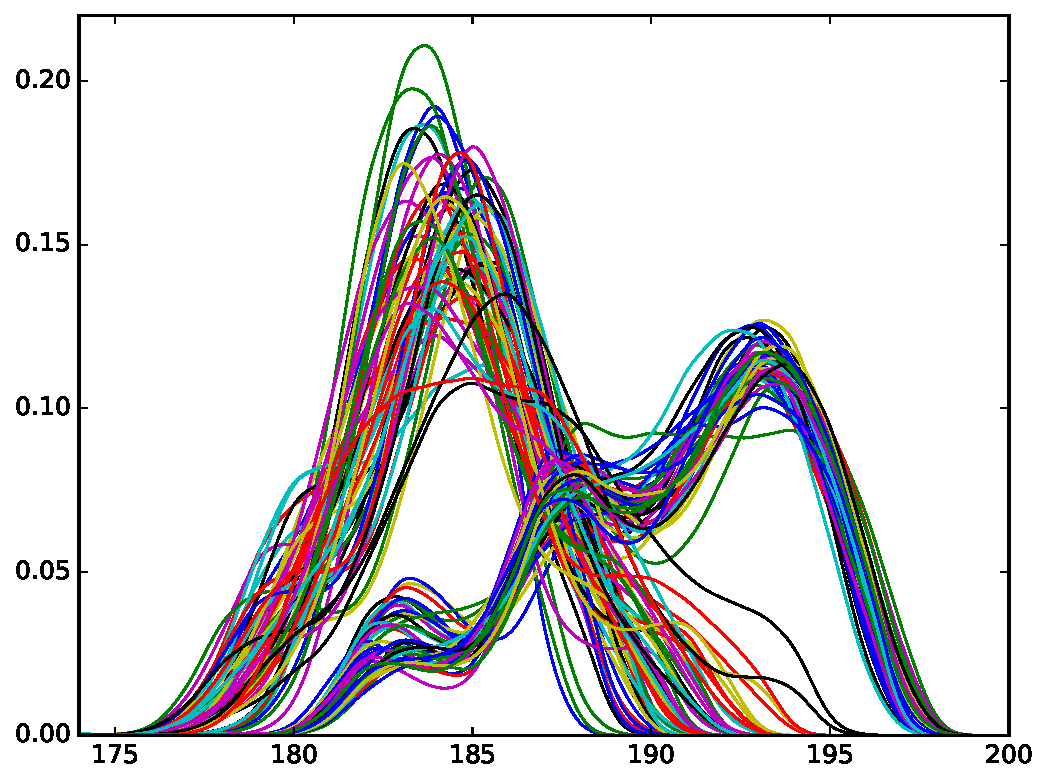
\includegraphics[width=\columnwidth]{figures/fig4/kde_pdf_sumindex}
\caption{Kernel density estimates (KDEs) of the probability density functions
(pdfs) across 100 trials of the \lstinline|sumindex| benchmark. Each curve is a
KDE formed from a trial of 10,000 consecutively gathered timing measurements.
Note that the data form two distinct clusters. A cursory investigation did not
reveal any inter-trial correlations that revealed a predictable preference for
which cluster would be observed.}
\label{fig:pdfsumindex}
\end{figure}

\subsection{The oracle function}
\label{sec:oracle}

Our heuristic takes as input an oracle function $\nu(t)$ that maps expected
runtimes to an optimal number of executions per measurement. While
Alg.~\ref{alg:tuning} does not directly describe $\nu(t)$, appropriate choices
for this function should have the following properties:

\begin{itemize}
    \item $\nu(t)$ has a discrete range $\{1, \dots, j\}$.
    \item $\nu(t)$ is monotonically decreasing, so that the longer the runtime, the fewer repetitions per measurement.
    \item $\frac{d\nu}{dt}|_{t \approx \tau_{\textrm{prec}}} \approx 0$,
    so that there is only weak dependence on the timer precision parameter,
    which may not be accurately known.
    \item $\frac{d\nu}{dt}|_{t \approx \tau_{\textrm{acc}}} \approx 0$,
    so that there is only weak dependence on the timer accuracy parameter,
    which may not be accurately known.
    \item $\nu(\tau_{\textrm{prec}}) \approx j$, so that benchmarks that take a     short time to run are not repeated more times than necessary to mitigate timer inaccuracy.
    \item $\nu(t \ge \tau_{\textrm{acc}}) \approx 1$, so that benchmarks that take a long time to run need not be repeated.
\end{itemize}

There are many functions that satisfy these criteria. One useful example takes
the form of the generalized logistic function:

\begin{equation}
\label{eq:glog}
    Y(t) = \floor*{1 + \frac{j - 1}{1 + e^{a (t - b \tau_{\textrm{acc}})}}}
\end{equation}
%
where reasonable values of $a$ and $b$ are approximately $0.005 < a \tau_{\textrm{prec}} < 0.02$ and $0.4 < b <
0.6$.

In practice, we have found that better results can be achieved by first
approximating $Y(t)$ with a lookup table, then modifying the lookup table based
on empirical observations. This was accomplished by examining many benchmarks
with a variety of known runtimes at different time scales, seeking for each
runtime the smallest $n$ value at which the minimum estimate appears to
converge to a lower bound (e.g.\ around $n = 250$ for the benchmark in
Fig.~\ref{fig:scaling}). Fig.~\ref{fig:oracle} plots both \eqref{eq:glog} and an
empirically obtained lookup table as potential oracle functions.

\begin{figure}
\centering
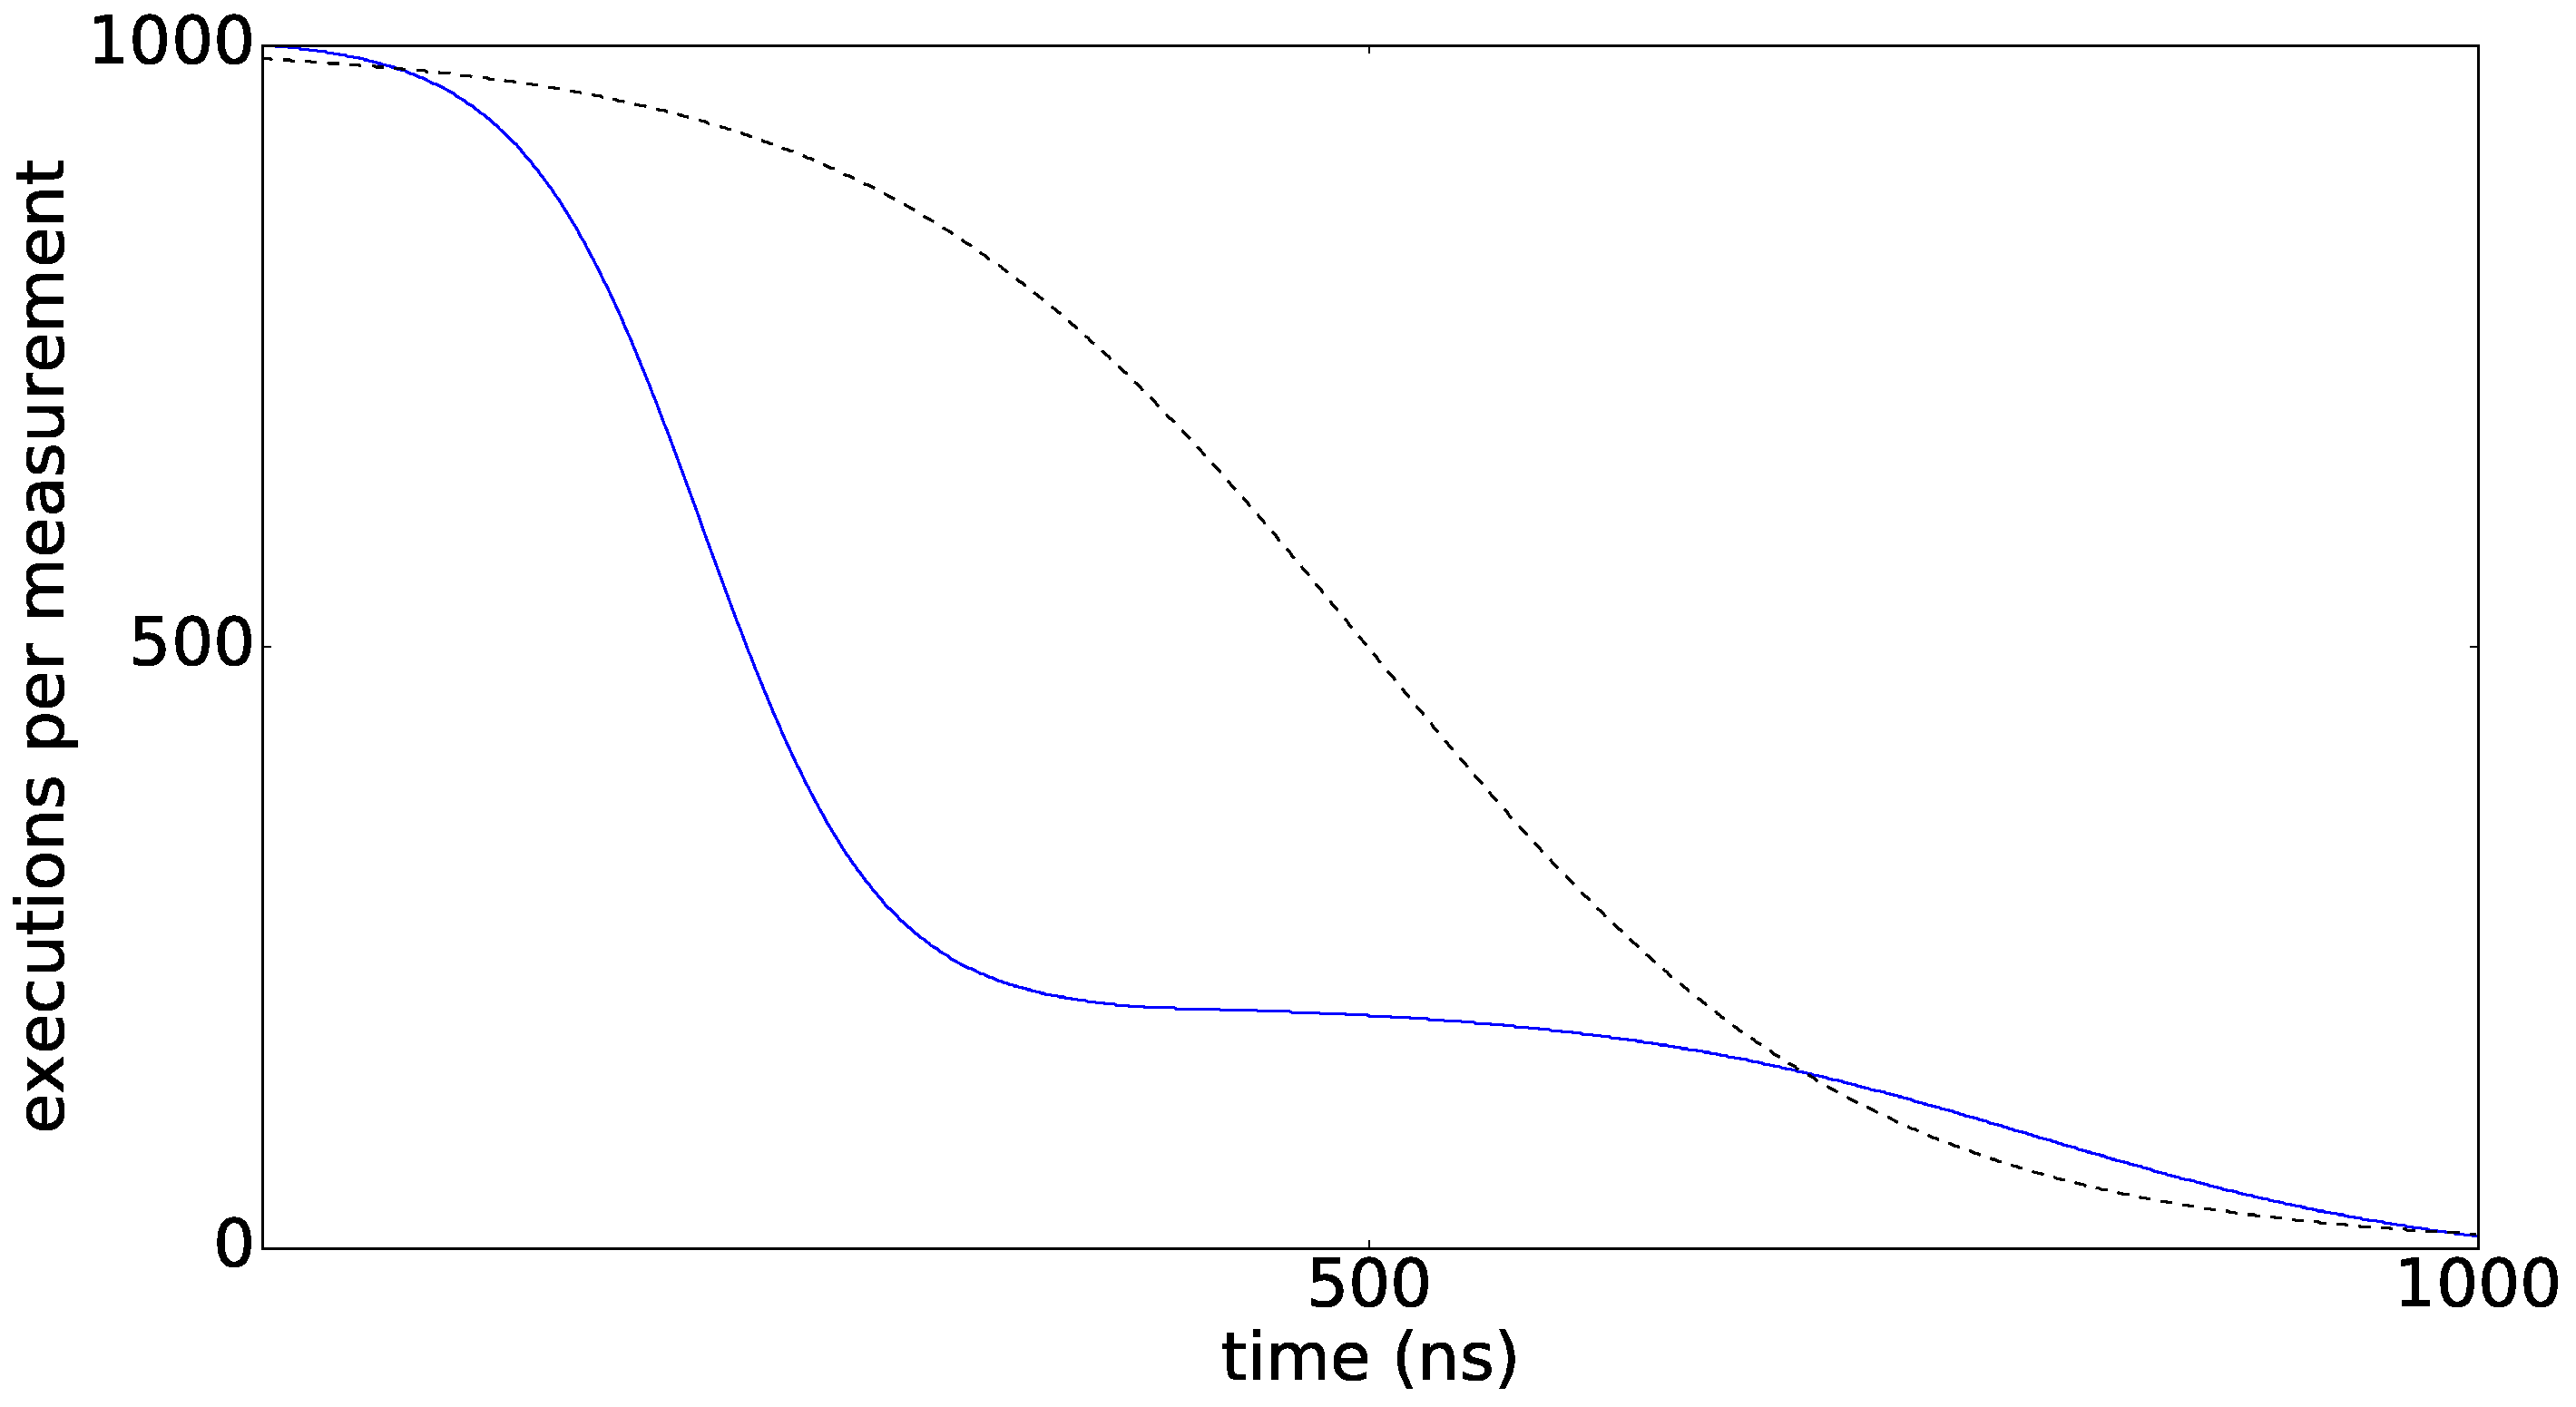
\includegraphics[width=\columnwidth]{figures/fig5/oracle}
\caption{Two possible oracle functions for $\nu(t)$ at $\tau_{\textrm{acc}} \approx 1000 \textrm{ns}$, $\tau_\textrm{prec} \approx 1 \textrm{ns}$.
The solid blue curve is an example of an empirically tuned lookup table, while
the dotted black curve is $Y(t)$ from Eq~\ref{eq:glog} with parameters $a =
0.009 / \tau_\textrm{prec}$ and $b = 0.5$.}
\label{fig:oracle}
\end{figure}

%%%%%%%%%%%%%%%%%%%%%%%%%%%%%%%%%%%%%%%%%%%%%%%%%%%%%%%%%%%%%%%%%%%%%%%%%%%%%%%%%%%%%%%%%%%%
%\section{The difficulties of hypothesis testing and a potential way forward}
%\label{sec:hypotesting}
%
%A logical next step would be to use our model to compare the timing estimates of two
%programs - or equivalently, two different versions of the same program - and provide to the
%reader an algorithm for calculating some measure of the statistical significance of the
%comparison, such as a confidence interval. Unfortunately, as mentioned in
%Section~\ref{sec:toughstats}, many common statistical tests are inapplicable to our
%model due to the non-i.i.d. (potentially even non-stationary) nature of benchmark timing
%measurements.
%
%For example, recall from Section~\ref{sec:model} that timing samples are drawn from a sum of
%scaled random variables following nonidentical Poisson binomial distributions. Though this
%technically constitutes a parameterized distribution, there are an overwhelming number of
%parameters to take into account. While it is possible that some benchmarks' timing
%distributions are feasibly derivable given extremely precise knowledge of the target program
%and execution environment, it is safe to say that, in practice, the excessive number of
%uncontrolled variables will generally render parametric hypothesis testing untenable.
%
%Often, nonparametric tests are used when it is infeasible to analytically derive the
%properties required by parametric tests. Consider the naive bootstrap, a popular
%resampling-based nonparametric method for hypothesis testing. In this method, new samples
%are randomly drawn from the original sample, in effect treating the original sample as an
%estimate of the original population so that an estimate for the distribution of a test
%statistic can be formed without prior knowledge of the original population's
%distribution~\cite{Efron1992}. While the naive bootstrap can sometimes succeed in the
%presence of non-identically distributed samples, it will generally fail when applied to
%correlated samples, since the resample will fail to capture correlations in the original
%sample~\cite{Mammen2012}. Luckily, statisticians have developed certain variants of these
%methods which are designed to work for correlated data.
%
%One of these variants is known as permutation testing, which can yield exact confidence
%intervals as long as the two samples being compared were drawn from populations following
%exchangeable distributions under the null hypothesis~\cite{Good2013}. The downside of
%permutation testing is that it can be immensely computationally expensive for large sample
%sizes, as it requires the test statistic to be calculated for many (if not all) permutations
%of the two original samples.
%
%Other resampling techniques, referred to as block resampling methods, preserve correlations
%by randomly drawing whole blocks of consecutive measurements from the original sample,
%rather than randomly drawing individual measurements. Well-known examples of block
%resampling methods include the block bootstrap~\cite{Kunsch1989}, the stationary
%bootstrap~\cite{Politis1994} and the block subsampling method~\cite{Politis1999}. The
%computational feasibility and robustness of block resampling methods in the presence of
%non-i.i.d., non-stationary, and even heteroskedastic behavior~\cite{Politis1999,Politis1997}
%make them promising candidates for use in automated statistical performance regression
%detection systems. The chief difficulty one faces when applying these methods is that they
%feature a low tolerance for suboptimal choices of configuration parameters. For example,
%these methods can fail to produce a uniform p-value distributions if the size of the
%resampled block is not chosen properly~\cite{Shao2013}. Additionally, in order to prevent
%degeneracy in the estimated distribution, one must apply a normalization coefficient to the
%test statistic~\cite{Politis1999}. This coefficient is derived from the rate of convergence
%of the statistic's variance with increasing sample size, which can depend on the original
%population's underlying distribution.
%
%In order to obviate the need for manual derivation of block sizes and normalization
%coefficients, statisticians have proposed several automatable, data-dependent procedures for
%selecting them~\cite{Politis2004,Bickel2008}. Furthermore, several augmentations have been
%devised that can increase the statistical power of block resampling methods under suboptimal
%or nontraditional choice of configuration parameters~\cite{Berg2010,Shao2013}. We believe
%that an investigation of the applicability of these procedures, and block resampling methods
%in general, could prove a fruitful avenue of future research for the study of statistical
%regression detection.
%
%%%%%%%%%%%%%%%%%%%%%%%%%%%%%%%%%%%%%%%%%%%%%%%%%%%%%%%%%%%%%%%%%%%%%%%%%%%%%%%%%%%%%%%%%%%%
\section{Implementation in Julia}
\label{sec:implementation}

The experimental methodology in this paper is implemented in the
\lstinline|BenchmarkTools| Julia
package\footnote{\url{https://github.com/JuliaCI/BenchmarkTools.jl}}. In
addition to the
\lstinline|BaseBenchmarks|\footnote{\url{https://github.com/JuliaCI/BaseBenchmarks.jl}}
and
\lstinline|Nanosoldier|\footnote{\url{https://github.com/JuliaCI/Nanosoldier.jl}}
packages, the \lstinline|BenchmarkTools| package implements the on-demand CI
benchmarking service used by core Julia developers to compare the performance
of proposed language changes with respect to over 1300 benchmarks. Since this
CI benchmarking service began in early 2016, it has caught and prevented the
introduction of dozens of serious performance regressions into Julia's standard
library (defining a ``serious'' regression as a $30\%$ or greater increase in a
benchmark's minimum execution time).

The benchmarks referenced in this paper are Julia benchmarks written and
executed using \lstinline|BenchmarkTools|. A brief description of each
benchmark is offered below:

\begin{itemize}
    \item The \lstinline|sumindex(a, inds)| benchmark sums over all
\lstinline|a[i]| for all \lstinline|i| in \lstinline|inds|. This test stresses
memory layout via element retrieval.
    \item The \lstinline|pushall!(a, b)| benchmark pushes elements from \lstinline|b| into
    \lstinline|a| one by one, additionally generating a random number at each iteration (the
    random number does not affect the output). This test stresses both random number
    generation and periodic reallocation that occurs as part of Julia's dynamic array
    resizing algorithm.
    \item The \lstinline|branchsum(n)| benchmark loops from \lstinline|1| to \lstinline|n|.
    If the loop variable is even, a counter is decremented. Otherwise, an inner loop is
    triggered which runs from \lstinline|1| to \lstinline|n|, in which another parity test
    is performed on the inner loop variable to determine whether to increment or decrement
    the counter. This test stresses periodically costly branching within loop iterations.
    \item The \lstinline|manyallocs(n)| allocates an array of \lstinline|n| elements, where
    each element is itself an array. The inner array length is determined by a random number
    from \lstinline|1| to \lstinline|n|, which is regenerated when each new array is
    constructed. However, the random number generator is reseeded before each generation so
    that the program is deterministic. This test stresses random number generation and
    the frequent allocation of arrays of differing length.
\end{itemize}

The mock benchmark suite referenced in this paper is hosted on GitHub at
\url{https://github.com/jiahao/paper-benchmark}.

%%%%%%%%%%%%%%%%%%%%%%%%%%%%%%%%%%%%%%%%%%%%%%%%%%%%%%%%%%%%%%%%%%%%%%%%%%%%%%%%%%%%%%%%%%%%
\section{Conclusion}
\label{sec:conclusion}

The complexities of modern hardware and software environments produce
variations in benchmark timings, with highly nonideal statistics, that
complicate the detection of performance regressions. Timing measurements taken
from real Julia benchmarks confirm the observations of many other authors
showing highly nonideal, even multimodal behavior, exhibited by even the
simplest benchmark codes.

Virtually all timing variations are delays caused by flushing cache lines, task
switching to background OS processes, or similar events. This simple
observation that variations are almost always one-sided led us to consider a
straightforward analysis based on a simple model for delays in a serial
instruction pipeline. Our results suggest that using the minimum estimator for
the true runtime of a benchmark, rather than the mean or median, is robust to
nonideal statistics and also provides the smallest error.  Our model also
revealed some behaviors that challenge conventional wisdom, such as simply
running a benchmark for longer, or repeating its execution many times, can
render the effects of external variation negligible, even as the error due to
timer inaccuracy is amortized.

Alg.~\ref{alg:tuning} presents an automatable heuristic for selecting the
minimum number of executions of a benchmark per measurement required to defeat
timer error. This strategy has been implemented in the
\lstinline|BenchmarkTools| Julia package, which is employed daily and on demand
as part Julia's continuous integration (CI) pipeline to evaluate the
performance effects of proposed changes to Julia's standard library in a fully
automatic fashion. \lstinline|BenchmarkTools| can also be used to test the
performance of user-authored Julia packages.


%%%%%%%%%%%%%%%%%%%%%%%%%%%%%%%%%%%%%%%%%%%%%%%%%%%%%%%%%%%%%%%%%%%%%%%%%%%%%%%%%%%%%%%%%%%%
\section*{Acknowledgment}
\label{sec:acknowledgement}

We thank the many Julia developers, in particular Andreas Noack and Steven G.
Johnson of MIT, for many insightful discussions.

This research was supported in part by the U.S. Army Research Office under
contract W911NF-13-D-0001, the Intel Science and Technology Center for Big
Data, and DARPA XDATA.

%%%%%%%%%%%%%%%%%%%%%%%%%%%%%%%%%%%%%%%%%%%%%%%%%%%%%%%%%%%%%%%%%%%%%%%%%%%%%%%%%%%%%%%%%%%%
\bibliography{biblio}
\bibliographystyle{IEEEtran}

% that's all folks
\end{document}
\grid
